\begin{exo}
  \donnee{Un serveur de calcul reçoit des requêtes à fréquence régulière. Elles sont traitées indépendamment les unes après les autres dans leur ordre d'arrivée. On suppose que le nombre de requêtes qui arrivent au serveur peut être modélisé par un processus de Poisson. Les requêtes sont envoyées vers le serveur à un
  \begin{center}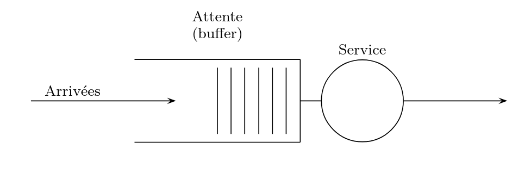
\includegraphics[scale=0.8]{ex2.png}\end{center}
}
	\begin{subexo}{}
	\end{subexo}
\end{exo}
